\documentclass[12pt,fleqn]{article}\usepackage{../common}
\begin{document}
Ders 5

Permutasyonlar

Bu derste bir anlamda lineer cebirin ruhunu gormeye baslayacagiz, sadece
vektorler degil artik vektor uzaylarina bakmaya baslayacagiz, yani daha
buyuk resme odaklanacagiz. Ayrica herhangi bir uzayin alt-uzaylarini
(subspace) inceleyecegiz. 

Simdi permutasyonlari hatirlayalim - permutasyon matrisi $P$ bir diger
matrisin satirlarini degis-tokus etmek icin kullaniliyordu. Bu isleme
ihtiyacimiz olacak, cunku, elimizde $Ax=b$ cozerken belki de (neredeyse)
mukemmel bir $A$ olsa da bazen mesela tek bir yerdeki sifir isi bozuyor
olabilir, onu yerinden oynatirsam, duzgun bir pivot elde edersem cozum
olacaktir, iste o zaman permutasyon kullanabilirim.

Peki $A=LU$ ile bir sistemi cozerken gerekebilecek permutasyonlar ile
alakasi nedir?

$A=LU$'nin ne oldugunu hatirlayalim, 

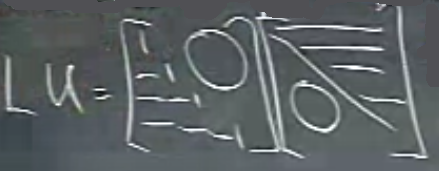
\includegraphics[height=3cm]{5_01.png}

Bu resme bakarsa, $LU$ baglaminda $P$ yoktur, daha dogrusu birim matristir
(identity matrix). 

Simdi bir dakika durup mesela Matlab [artik Python] lineer cebir
kutuphanelerinin cozumu nasil yaptigini dusunelim. Bu kutuphaneler pivot'in
sifir olup olmadigina bakarlar, ki herhangi bir insan da bunu yapar, ayrica
pivot'in ``yeterince buyuk olup olmadigina da'' bakilir, cunku sifira
yakin, cok kucuk pivotlar sayisal hesap baglaminda kotudur. Bu durumda
kutuphaneye ``coz'' dedigimizde kodun arka planda satir degis-tokuslari
yaptigini gorururuz, bu degisimler pur matematiksel olarak gerekli
olmayabilirler, ama hesap / sayisal acidan gereklidirler. 

Nihai olarak satir degisimini iceren eliminasyon sudur:

$$ PA = LU $$

6:03
















\end{document}
